\documentclass{article}
\usepackage{ctex}
\usepackage{geometry}
\geometry{a4paper,scale=0.9}
\usepackage{enumitem}
\usepackage{amsmath}
\usepackage{amssymb}
\usepackage{graphicx}
\usepackage{float}

\title{HW02}
\author{PB19071405\ 王昊元}
\date{2022 年 3 月 28 日}


\begin{document}
    \pagestyle{empty}

    \maketitle
    \thispagestyle{empty}  % for maketitle

    \begin{enumerate}[label=\arabic*.]
        \item \begin{enumerate}[label=\alph*.]
            \item 写后读-RAW\ 读后写-WAR\ 写后写-WAW\\
            \begin{tabular}{|c|c|c|}
                \hline
                寄存器 & 指令 & 类型 \\
                \hline
                R1 & \textcircled{1} \textcircled{2} & RAW、WAW \\
                \hline
                R1 & \textcircled{1} \textcircled{3} & RAW \\
                \hline
                R2 & \textcircled{1} \textcircled{4} & WAR \\
                \hline
                R1 & \textcircled{2} \textcircled{3} & RAW \\
                \hline
                R2 & \textcircled{3} \textcircled{4} & WAR \\
                \hline
                R2 & \textcircled{4} \textcircled{5} & RAW \\
                \hline
                R4 & \textcircled{5} \textcircled{6} & RAW \\
                \hline
            \end{tabular}
            \item 时序如下:\\
            \scalebox{0.7}{
            \begin{tabular}{lcccccccccccccccccc}
                \hline
                & 1 & 2 & 3 & 4 & 5 & 6 & 7 & 8 & 9 & 10 & 11 & 12 & 13 & 14 & 15 & 16 & 17 & 18 \\
                \hline
                LD\ R1,\ 0(R2) & IF & ID & EX & MEM & WB &&&&&&&&&&&&& \\
                DADDI\ R1,\ R1,\ \#1 & & IF & s & s & ID & EX & MEM & WB &&&&&&&&&& \\
                SD\ 0(R2),\ R1 & & & & & IF & s & s & ID & EX & MEM & WB &&&&&&& \\
                DADDI\ R2,\ R2,\ \#4 & & & & & & & & IF & ID & EX & MEM & WB &&&&&& \\
                DSUB\ R4,\ R3,\ R2 & & & & & & & & & IF & s & s & ID & EX & MEM & WB &&& \\
                BNEZ\ R4,\ Loop & & & & & & & & & & & & IF & s & s & ID & EX & MEM & WB \\
                &&&&&&&&&&&&&&&&&& \\
                LD\ R1,\ 0(R2) &&&&&&&&&&&&&&&&& IF & ID \\
                \hline
            \end{tabular}}

            所需周期: $98 \times 16 + 18 = 1586$
            \item 时序如下:\\
            \scalebox{0.8}
            {
                \begin{tabular}{lcccccccccccccc}
                    \hline
                    & 1 & 2 & 3 & 4 & 5 & 6 & 7 & 8 & 9 & 10 & 11 & 12 & 13 & 14 \\
                    \hline
                    LD\ R1,\ 0(R2) & IF & ID & EX & MEM & WB &&&&&&&&& \\
                    DADDI\ R1,\ R1,\ \#1 && IF & ID & s & EX & MEM & WB &&&&&&& \\
                    SD\ 0(R2),\ R1 &&& IF & s & ID & EX & MEM & WB &&&&&& \\
                    DADDI\ R2,\ R2,\ \#4 &&&&& IF & ID & EX & MEM & WB &&&&& \\
                    DSUB\ R4,\ R3,\ R2 &&&&&& IF & ID & EX & MEM & WB &&&& \\
                    BNEZ\ R4,\ Loop &&&&&&& IF & s & ID & EX & MEM & WB && \\
                    (the inst after \textcircled{6}) &&&&&&&&& IF & s & s & s & s & \\
                    LD\ R1,\ 0(R2) &&&&&&&&&& IF & ID & EX & MEM & WB \\
                    \hline
                \end{tabular}
            }

            % 认为最后一次循环的 EX 阶段判断 R4 寄存器与 0 的关系代表着循环结束,则
            所需周期: $98 \times 9 + 12 = 894$

            \item 时序如下:\\
            \scalebox{0.8}
            {
                \begin{tabular}{lccccccccccccc}
                    \hline
                    & 1 & 2 & 3 & 4 & 5 & 6 & 7 & 8 & 9 & 10 & 11 & 12 & 13 \\
                    \hline
                    LD\ R1,\ 0(R2) & IF & ID & EX & MEM & WB &&&&&&&& \\
                    DADDI\ R1,\ R1,\ \#1 && IF & ID & s & EX & MEM & WB &&&&&& \\
                    SD\ 0(R2),\ R1 &&& IF & s & ID & EX & MEM & WB &&&&& \\
                    DADDI\ R2,\ R2,\ \#4 &&&&& IF & ID & EX & MEM & WB &&&& \\
                    DSUB\ R4,\ R3,\ R2 &&&&&& IF & ID & EX & MEM & WB &&& \\
                    BNEZ\ R4,\ Loop &&&&&&& IF & s & ID & EX & MEM & WB & \\
                    % &&&&&&&&&&&&& \\
                    \\
                    LD\ R1,\ 0(R2) &&&&&&&&& IF & ID & EX & MEM & WB \\
                    \hline
                \end{tabular}
            }

            所需周期: $98 \times 8 + 12 = 796$
        \end{enumerate}

        \item 时空图如下:\\
        \begin{figure}[H]
            \centering
            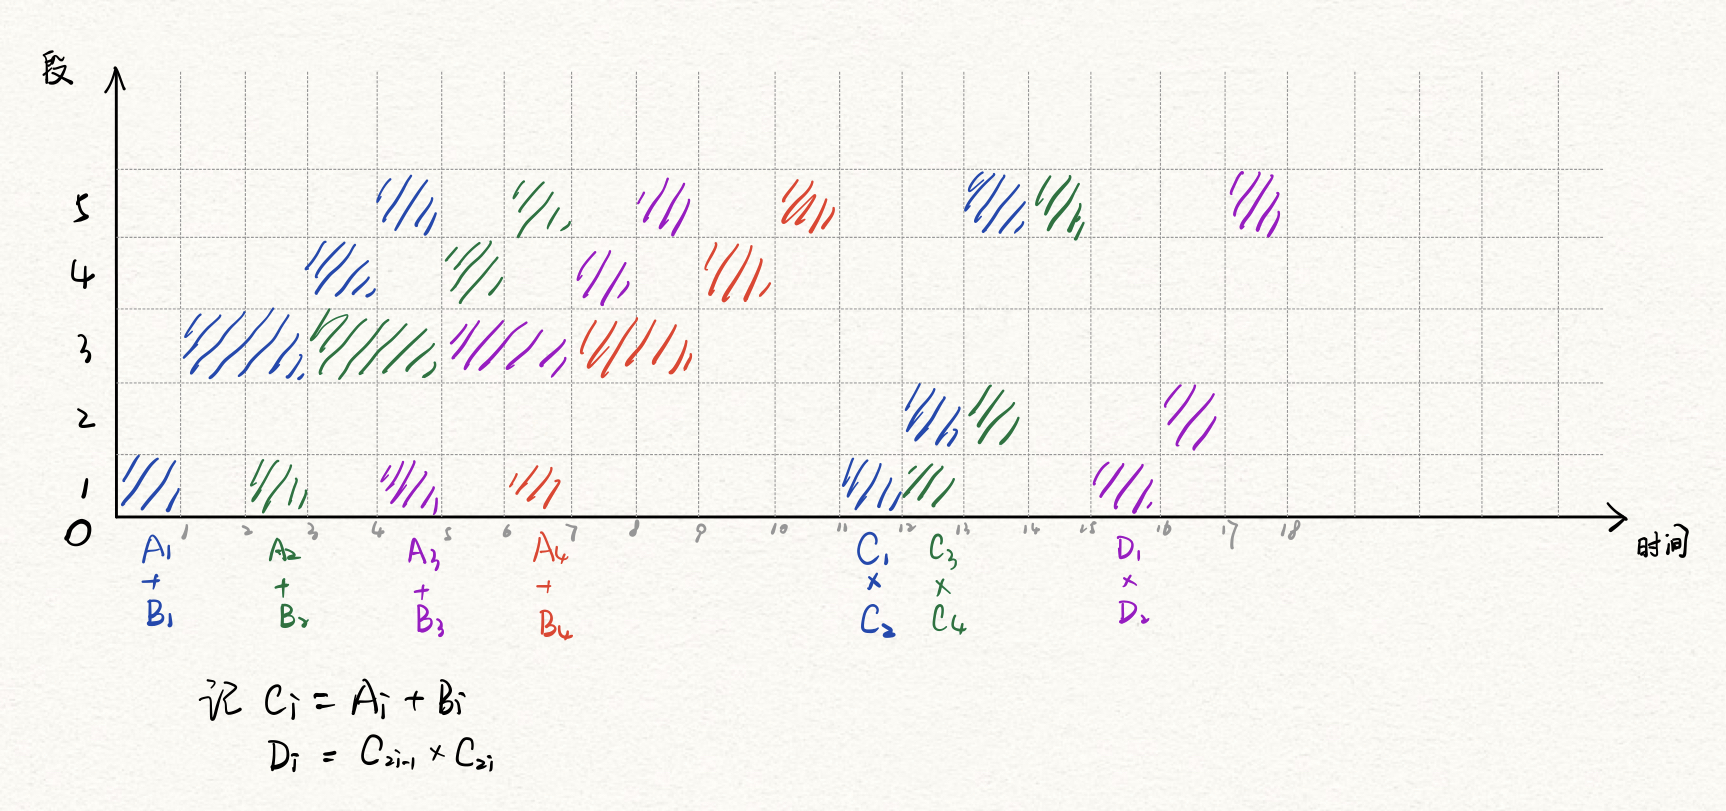
\includegraphics[width=0.7\textwidth]{fig/hw02_q2_fig1.jpg}
            \caption{时空图}
        \end{figure}

        吞吐率: $TP = \frac{7}{18\Delta t}$

        加速比: $S = \frac{4 \times 5\Delta t + 3 \times 3\Delta t}{18\Delta t} \approx 1.61$

        效率: $E = \frac{4 \times 5\Delta t + 3 \times 3\Delta t}{5 \times 18\Delta t} \approx 0.322$

        \item \begin{enumerate}[label=\alph*.]
            \item 仅考虑数据相关时,5级流水线的 $CPI_1 = \frac{6}{5}$,12级流水线的 $CPI_2 = \frac{11}{8}$。\\
            则加速比为 $\frac{I \times CPI_1 \times T_1}{I \times CPI_2 \times T_2} = \frac{\frac{6}{5} \times 1}{\frac{11}{8} \times 0.6} = \frac{16}{11} \approx 1.45 $
            \item 在考虑分支预测错误导致的 stall 时, 预测指令预测失败导致的额外周期即为相较于仅考虑数据相关时的额外CPI,即\\
            $CPI^\prime_1 = CPI_1 + 0.05 \times 0.2 \times 2 = \frac{61}{50} = 1.22$\\
            $CPI^\prime_2 = CPI_2 + 0.05 \times 0.2 \times 5 = 1.425$
        \end{enumerate}
    \end{enumerate}

\end{document}